\chapter{Bibliotecas}
Todas las bibliotecas usadas son de código abierto, así como también
todo el código desarrollado con ellas. Se marca una clara diferencia
con las políticas de las empresas que venden \gls{tcoa} las cuales no
permiten por derechos de autor cualquier modificación o conocimiento
interno tanto de la máquina como de su software. Normalmente las
actualizaciones del software de una \gls{tcoa} suelen ser gratuitas
pero otras de mayor importancia y/o críticas pueden llegar a costar
desde miles de euros hasta cientos de miles. \\
Un objetivo entre otros de este proyecto es tratar de romper con la
dependencia costosa de actualizaciones con estas compañías y crear de
0 nuevas bibliotecas y software de manera personalizada, abierta y
transparente a disposición de los oftalmólogos y adaptarlo a sus
necesidades incipientes en sus investigaciones.

\section{Bibliotecas de terceros}
\subsection{NumPy}
\begin{figure}[H]
  
\includegraphics[scale=0.5]{imagenes/logos/numpy_logo.png}
\end{figure}
Biblioteca principal para cálculo científico con
\emph{Python}. Destaca por:
\begin{itemize}
\item Matrices N-dimensionales para albergar las imágenes.
\item Operaciones de álgebra lineal para las matrices.
\item Integración con el resto de bibliotecas del proyecto.
\end{itemize}

\subsection{matplotlib}
\begin{figure}[H]
  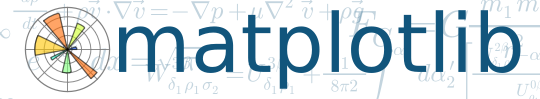
\includegraphics[scale=0.2]{imagenes/logos/matplotlib_logo.png}
\end{figure}
Biblioteca para dibujar gráficas en 2D y 3D en \emph{Python}. Muy
usada en el campo de visión computerizada para la visualización de
histogramas.

\subsection{OpenCV}
\begin{figure}[H]
  \hspace*{1.4cm}
  
\includegraphics[scale=0.2]{imagenes/logos/opencv_logo.png}
\end{figure}
Biblioteca de visión computerizada escrita en C++ y diseñada para
permitir su utilización en aplicaciones de tiempo real. Proporciona:
\begin{itemize}
\item Integración precisa con \emph{Python} y \emph{NumPy}.
\item Contiene funciones y algoritmos aplicables a todas las áreas de
  visión computerizada, especialmente para imágenes en 2D.
\item Creación de interfaces gráficas con paneles para facilitar la
  interacción con las técnicas aplicadas a las imágenes.
\end{itemize}

\subsection{SimpleCV}
\begin{figure}[H]
  \hspace*{1.7cm}
  
\includegraphics[scale=0.3]{imagenes/logos/simplecv_logo.png}
\end{figure}
Biblioteca de visión computerizada escrita en \emph{Python} sobre
\emph{OpenCV} que provee varios algoritmos complejos con una interfaz
mucho más simple que OpenCV\@.

\section{Bibliotecas propias}

Bibliotecas desarrolladas por y para el proyecto. Son envolturas a
otras bibliotecas con el objetivo de adaptarlas a las necesidades
surgidas con las \gls{tcoa}.

\subsection{Envoltura del módulo argparse}
Biblioteca escrita para facilitar la integración con el módulo
\emph{argparse} de la biblioteca estándar de \emph{Python} e
incorporar procesamiento de argumentos por consola como:
\begin{itemize}
\item Modo depuración.
\item Procesamiento de imágenes individuales.
\item Procesamiento de carpetas de imágenes.
\end{itemize}

\subsection{Extracción de zonas de interés}
Biblioteca que se encarga de extraer la región que se va a estudiar de
una \gls{tcoa}.

\subsection{Corrección de la inclinación}
Biblioteca que corrige la inclinación de las \gls{tcoa}, poniéndolas
horizontales si no lo están.

\footnotetext{Todos los logos de terceros mostrados
  en este capítulo pertenecen a sus respectivos autores y están
  protegidos por las leyes de derechos de autor}
